\section{Vincoli}
\subsection{Vincoli Tecnologici}\label{chap:vincoli tec}
{\company} non ha specificato vincoli in merito alle tecnologie da utilizzare, tuttavia essendo che lo scopo del progetto è quello di 
sviluppare un modulo per un'applicazione già esistente, i vincoli tecnologici impliciti sono di utilizzare gli stessi framework già 
impiegati per lo sviluppo in modo da eventualmente poter integrare il modulo all'interno dell'app che viene commercializzata.\\
Non esistono divieti riguardo l'introduzione di nuove tecnologie, come descritto nel capitolo \ref{chap:strategia} uno degli obiettivi 
che l'azienda intende raggiungere con il progetto di stage e quello di (se implementate) valutare il beneficio che nuove librerie, framework 
e tecnologie portano per poter innovare e crescere.\\
Anche per quanto riguarda le tecnologie da utilizzare non ho avuto vincoli espliciti, a parte per quanto riguarda l'utilizzo di BitBucket 
come piattaforma in cui conservare il codice.\\
Le tecnologie utilizzate per sviluppare il modulo agenti sono:
\begin{itemize}
    \item \textbf{Visual Studio}: per lo sviluppo delle \gls{api}, Visual Studio implementa molti strumenti per 
          il \textit{debug} del codice e permette di gestire facilmente l'installazione dei pacchetti necessari. 
          Inoltre è particolarmente utile per lo sviluppo in C\# in quanto dispone di funzioni per l'auto completamento 
          del codice velocizzando lo sviluppo e dell'aggiornamento automatico degli \textit{import};
    \item \textbf{Visual Studio Code}: per lo sviluppo del \textit{front-end} per via delle molte estensioni 
          disponibili a supporto dello sviluppo in React (come Prettier, che permette una formattazione uniforme 
          per il codice).
    \item \textbf{Computer con Windows 10}: scelto in alternativa al Mac per via della mia esperienza pregressa 
          con Windows, evitando di dover imparare ad usare un nuovo sistema operativo oltre alle nuove tecnologie necessarie;
    \item \textbf{\textit{Smartphone} Android}: per il \textit{testing} dell'applicazione;
    \item \textbf{BitBucket}: per conservare il mio codice all' interno di un \textit{branch} del progetto ed avere a 
        disposizione le funzionalità di Git;
    \item \textbf{Confluence}: per conservare la documentazione creata;
    \item \textbf{Word}: per creare la documentazione tecnica, visto che permette di creare velocemente e semplicemente un 
          documento in modo che sia facilmente consultabile e modificabile;
    \item \textbf{Figma}: per creare il manuale utente. Figma permette una gestione dello stile più precisa e personalizzabile
          di Word ma richiede molto più tempo per creare un documento. Si ottiene quindi un impatto grafico migliore, poco utile nel 
          caso di un documento tecnico, apprezzabile nel caso di un documento destinato all'utente finale;
    \item \textbf{Servizio di posta elettronica}: per ricevere gli annunci aziendali;
    \item \textbf{SQL Server Management Studio (SSMS)}: per operare sul \textit{database} usato per lo sviluppo dell'
          applicazione;
    \item \textbf{Swagger}: per testare manualmente le \gls{api} e valutarne il corretto funzionamento.
\end{itemize}
Cito per completezza anche 3CX tra le tecnologie che mi sono state fornite. Tuttavia, non ho mai avuto la necessità di utilizzarla, 
poiché ho avuto la possibilità di confrontarmi personalmente con gli sviluppatori e il tutor aziendale. Inoltre, durante 
il mio stage, il 
\textit{meeting} mensile generale è stato annullato, quindi non ho potuto partecipare alla video chiamata.\\
I \textit{framework} e le librerie utilizzate sono:
\begin{itemize}
    \item \textbf{React Native}: \textit{framework} che permette di sviluppare applicazioni Android e iOS utilizzando il 
    \textit{framework} React. Questo contiene funzionalità specifiche per i dispositivi \textit{mobile} a differenza di 
    React che viene utilizzato principalmente per sviluppare siti \textit{web}, e permette di scrivere e mantenere un unico 
    codice funzionante per entrambi i sistemi operativi evitando la necessità di avere sviluppatori specializzati nello 
    sviluppo Android e altri specializzati nello sviluppo iOS;
    \item \textbf{React Native Paper}: libreria di componenti per le interfacce;
    \item \textbf{React Native Navigation}: libreria per la gestione della navigazione tra le \textit{view};
    \item \textbf{ASP.NET Core}: \textit{framework open source} moderno per lo sviluppo di applicazioni connesse ad \textit{internet}, 
          utilizzato nel mio caso per lo sviluppo delle \gls{api} necessarie.
\end{itemize}

\subsection{Vincoli Temporali}\label{chap:vincoli temporali}
\begin{figure}[H]
    \centering
    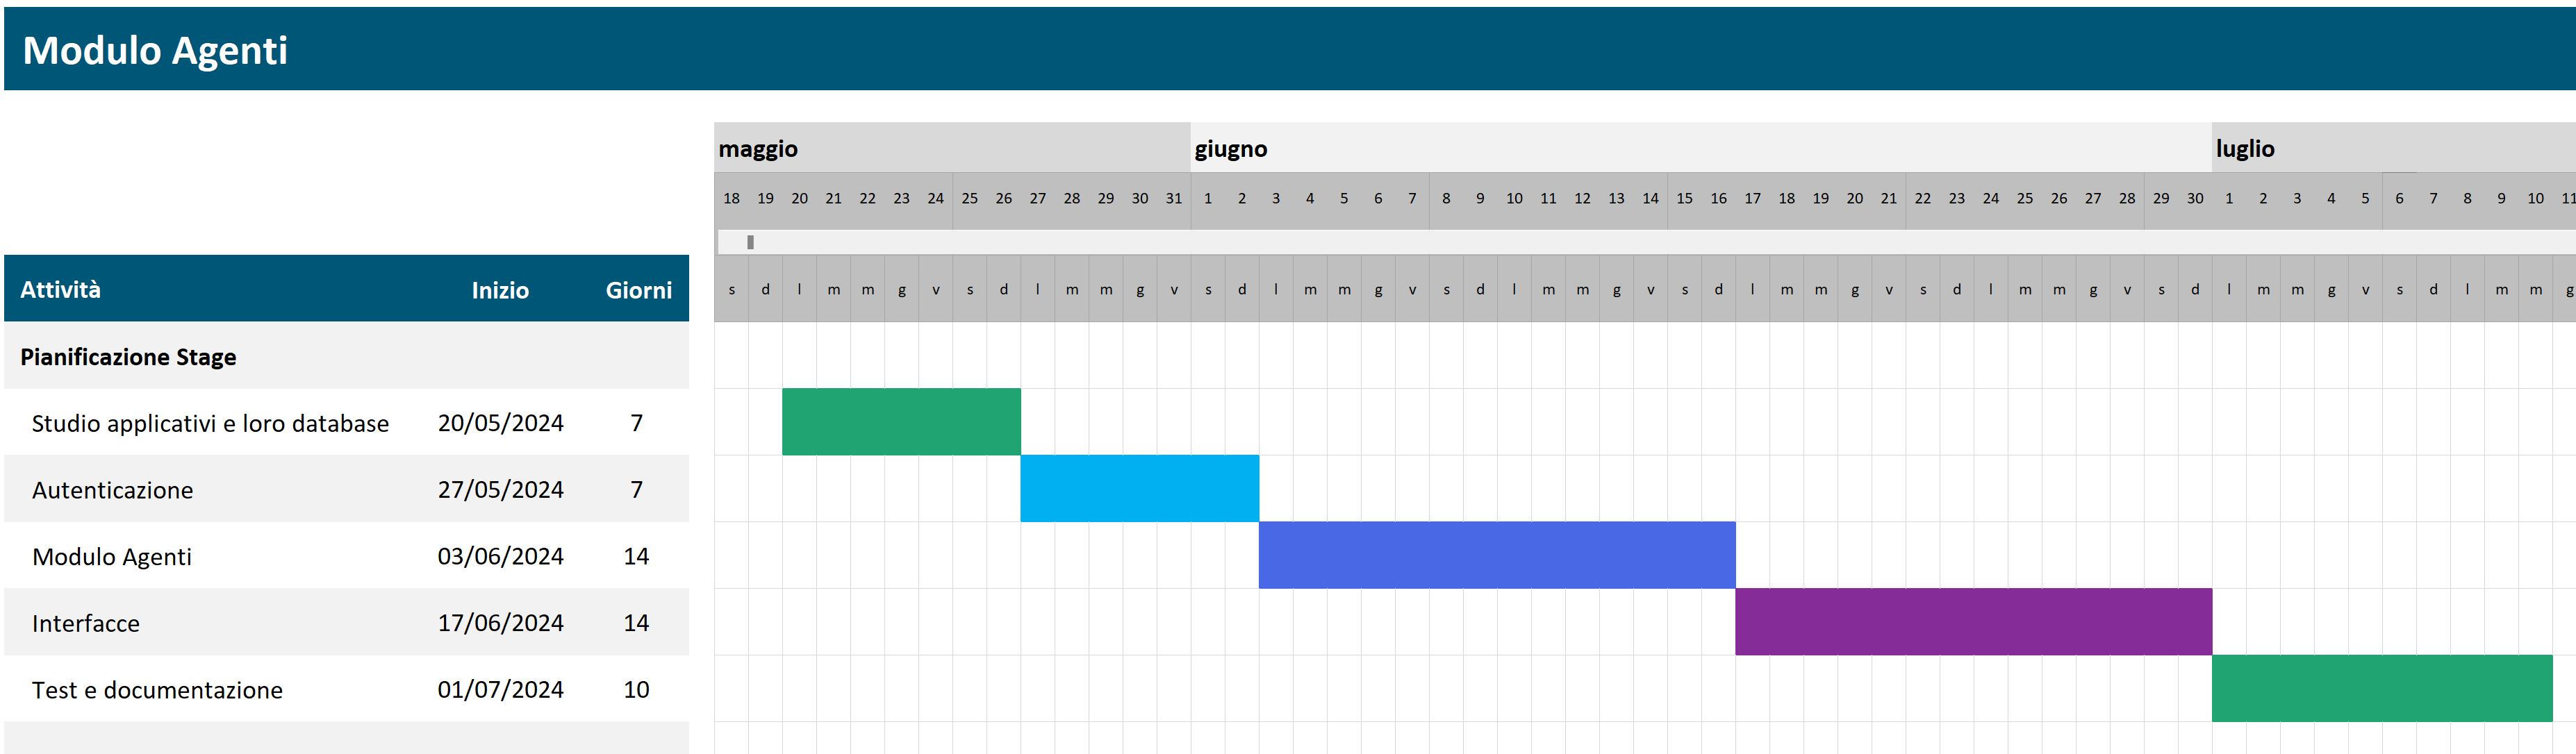
\includegraphics[alt={Pianificazione attività di stage}, width=\textwidth]{img/gantt pianificazione.png}
    \caption[Pianificazione attività di stage]
            {Pianificazione attività di stage}
    \label{fig:pianificazione stage}
\end{figure}

Quello mostrato in figura \ref{fig:pianificazione stage} è la pianificazione delle mie attività di stage 
così come è riportata nel piano di lavoro, concordato tra me e il tutor aziendale e approvato dal relatore.\\
La prima attività, della durata di una settimana, è lo \textbf{studio degli applicativi e del database}, ovvero 
lo studio delle tecnologie utilizzate e del codice sorgente.\\
Quindi la seconda attività, della durata di una settimana, prevede di iniziare lo sviluppo partendo dalla \textbf{modifica 
della \gls{api} di autenticazione} in modo da permettere il \textit{login} del nuovo tipo di utente di tipo agente.\\
La terza attività, della durata di due settimane, prevede lo \textbf{sviluppo del modulo agenti}: le \gls{api} necessarie e la modifica del \textit{front-end}.\\
La penultima attività, della durata di due settimane, prevede la \textbf{modifica delle interfacce}, creazione dei componenti, 
definizione dello stile della UI (\textit{User Interface}) e ottimizzazione per \textit{tablet};\\
L'ultima attività, della durata di dieci giorni, prevede la \textbf{creazione della documentazione tecnica e operativa, 
del manuale utente e il \textit{testing} dell'applicazione}.